\documentclass[table]{beamer}
%[]中可以使用draft、handout、screen、transparency、trancompress、compress等参数

%指定beamer的模式与主题
\mode<presentation>
{
  \usetheme{Madrid}
%\usetheme{Boadilla}
%\usecolortheme{default}
%\usecolortheme{orchid}
%\usecolortheme{whale}
%\usefonttheme{professionalfonts}
}

%\usetheme{Madrid}
%这里还可以选择别的主题:Bergen, Boadilla, Madrid, AnnArbor, CambridgeUS, Pittsburgh, Rochester, Warsaw, ...
%有导航栏的Antibes, JuanLesPins, Montpellier, ...
%有内容的Berkeley, PaloAlto, Goettingen, Marburg, Hannover, ...
%有最小导航栏的Berlin, Ilmenau, Dresden, Darmstadt, Frankfurt, Singapore, Szeged, ...
%有章和节表单的Copenhagen, Luebeck, Malmoe, Warsaw, ...

%\usecolortheme{default}
%设置内部颜色主题(这些主题一般改变block里的颜色);这个主题一般选择动物来命名
%这里还可以选择别的颜色主题,如默认的和有特别目的的颜色主题default,structure,sidebartab,全颜色主题albatross,beetle,crane,dove,fly,seagull,wolverine,beaver

%\usecolortheme{orchid}
%设置外部颜色主题(这些主题一般改变title里的颜色);这个主题一般选择植物来命名
%这里还可以选择别的颜色主题,如默认的和有特别目的的颜色主题lily,orchid,rose

%\usecolortheme{whale}
%设置字体主题;这个主题一般选择海洋动物来命名
%这里还可以选择别的颜色主题,如默认的和有特别目的的颜色主题whale,seahorse,dolphin

%\usefonttheme{professionalfonts}
%类似的还可以定义structurebold,structuresmallcapsserif,professionalfonts

% 控制 beamer 的风格,可以根据自己的爱好修改
%\usepackage{beamerthemesplit} %使用 split 风格
%\usepackage{beamerthemeshadow} %使用 shadow 风格
%\usepackage[width=2cm,dark,tab]{beamerthemesidebar}

%插入音标
%\usepackage{tipa}
%\AtBeginDocument{
  %\renewcommand\textipa{\fontencoding{T3}\selectfont}
%}
%\AtBeginDocument{
  %\renewcommand\textipa[2][r]{{\fontfamily{cm#1}\tipaencoding #2}}
%}
%\renewenvironment{IPA}[1][r]
 %{\fontfamily{cm#1}\tipaencoding}
 %{}

% 设定英文字体
%\usepackage{fontspec}
% Fix bugs for fontspec in TeXLive2015
\ifdefined\suppressfontnotfounderror
  \expandafter\let\csname xetex_suppressfontnotfounderror:D\endcsname
    \suppressfontnotfounderror
\else
  \expandafter\let\csname xetex_suppressfontnotfounderror:D\endcsname
    \luatexsuppressfontnotfounderror
\fi
\usepackage[no-math]{fontspec}
\setmainfont{Times New Roman}
\setsansfont{Arial}
\setmonofont{Courier New}

% 设定中文字体
\usepackage[BoldFont,SlantFont,CJKchecksingle,CJKnumber]{xeCJK}
%\setCJKmainfont[BoldFont={Adobe Heiti Std},ItalicFont={Adobe Kaiti Std}]{Adobe Song Std}
\setCJKmainfont[BoldFont={Adobe Heiti Std},ItalicFont={Adobe Kaiti Std}]{WenQuanYi Micro Hei}
\setCJKsansfont{Adobe Heiti Std}
\setCJKmonofont{Adobe Fangsong Std}
\punctstyle{hangmobanjiao}

\defaultfontfeatures{Mapping=tex-text}
\usepackage{xunicode}
\usepackage{xltxtra}

\XeTeXlinebreaklocale "zh"
\XeTeXlinebreakskip = 0pt plus 1pt minus 0.1pt

\usepackage{setspace}
\usepackage{colortbl,xcolor}
\usepackage{hyperref}
%\hypersetup{xetex,bookmarksnumbered=true,bookmarksopen=true,pdfborder=1,breaklinks,colorlinks,linkcolor=blue,filecolor=black,urlcolor=cyan,citecolor=green}
\hypersetup{xetex,bookmarksnumbered=true,bookmarksopen=true,pdfborder=1,breaklinks,colorlinks,linkcolor=cyan,filecolor=black,urlcolor=blue,citecolor=green}

% 插入图片
\usepackage{graphicx}
\graphicspath{{figures/}}
% 图文混排
%\usepackage{picins}
\usepackage{floatflt}

% 可能用到的包
\usepackage{amsmath,amssymb}
%插入多媒体
%\usepackage{media9}
%\usepackage{movie15}
\usepackage{multimedia}
\usepackage{multicol}
\usepackage{multirow}

% 定义一些自选的模板,包括背景、图标、导航条和页脚等,修改要慎重
% 设置背景渐变由10%的红变成10%的结构颜色
%\beamertemplateshadingbackground{red!10}{structure!10}
%\beamertemplatesolidbackgroundcolor{white!90!blue}
% 使所有隐藏的文本完全透明、动态,而且动态的范围很小
\beamertemplatetransparentcovereddynamic
% 使itemize环境中变成小球,这是一种视觉效果
\beamertemplateballitem
% 为所有已编号的部分设置一个章节目录,并且编号显示成小球
\beamertemplatenumberedballsectiontoc
% 将每一页的要素的要素名设成加粗字体
\beamertemplateboldpartpage

% item逐步显示时,使已经出现的item、正在显示的item、将要出现的item呈现不同颜色
\def\hilite<#1>{
 \temporal<#1>{\color{gray}}{\color{blue}}
    {\color{blue!25}}
}

\renewcommand{\today}{\number\year 年 \number\month 月 \number\day 日}

%五角星
\usepackage{MnSymbol}

%去除图表标题中的figure等
\usepackage{caption}
\captionsetup{labelformat=empty,labelsep=none}

\usepackage{tabu}
\usepackage{multirow}
%表格自动换行
\usepackage{tabularx} 

% 千分号
%\usepackage{textcomp}

%罗马数字
\makeatletter
\newcommand{\rmnum}[1]{\romannumeral #1}
\newcommand{\Rmnum}[1]{\expandafter\@slowromancap\romannumeral #1@}
\makeatother

%分栏
\usepackage{multicol}

%\usepackage{enumitem}
%\usepackage{enumerate}

%键盘
\usepackage{keystroke}

%插入源代码
\usepackage{listings}
\lstset{
  language=perl,                  % 程序语言名称:TeX, Perl, R, sh, bash, Awk
  basicstyle=\normalsize\tt,      %\tt指monospace字体族,程序源代码使用此族字体表示更加美观
  numbers=left,                   % 行号位置(左侧)
  numberstyle=\small,             % 行号字体的字号
  stepnumber=1,                   % 行号的显示步长
  numbersep=5pt,                  % 行号与代码间距
  backgroundcolor=\color{white},  % 背景色;需要 \usepackage{color}
  showspaces=false,               % 不显示空格
  showstringspaces=false,         % 不显示代码字符串中的空格标记
  showtabs=false,                 % 不显示 TAB
  tabsize=4, 
  frame=shadowbox,                % 把代码用带有阴影的框圈起来
  captionpos=b,                   % 标题位置
  breaklines=true,                % 对过长的代码自动断行
  breakatwhitespace=false,        % 断行只在空格处
  extendedchars=false,            % 解决代码跨页时,章节标题,页眉等汉字不显示的问题
  %escapeinside={\%*}{*},         % 跳脱字符,添加注释,暂时离开 listings 
  %escapeinside=``,
  commentstyle=\color{red!50!green!50!blue!50}\tt,  %浅灰色的注释
  rulesepcolor=\color{red!20!green!20!blue!20},     %代码块边框为淡青色
  keywordstyle=\color{blue!70}\bfseries\tt,         %代码关键字的颜色为蓝色,粗体
  identifierstyle=\tt,
  stringstyle=\tt,                % 代码字符串的特殊格式
  keepspaces=true,
  breakindent=1em,
  %breakindent=22pt,
  %breakindent=4em,
  breakautoindent=true,
  flexiblecolumns=true,
  aboveskip=1em,                  %代码块边框
  xleftmargin=2em,
  xrightmargin=2em
}

%\setbeamercolor{alerted text}{fg=magenta}
\setbeamercolor{bgcolor}{fg=yellow,bg=cyan}
%\setbeamercolor{itemize/enumerate body}{fg=green}

\begin{document}

%\includeonlyframes{current}

\logo{
\includegraphics[height=0.08\textwidth]{tijmu.png}}

% 在每个Section前都会加入的Frame
\AtBeginSection[]
{
  \begin{frame}<beamer>
    %\frametitle{Outline}
    \frametitle{教学提纲}
    \setcounter{tocdepth}{3}
    \begin{multicols}{2}
      \tableofcontents[currentsection,currentsubsection]
      %\tableofcontents[currentsection]
    \end{multicols}
  \end{frame}
}
% 在每个Subsection前都会加入的Frame
\AtBeginSubsection[]
{
  \begin{frame}<beamer>
%%\begin{frame}<handout:0>
%% handout:0 表示只在手稿中出现
    \frametitle{教学提纲}
    \setcounter{tocdepth}{3}
    \begin{multicols}{2}
    \tableofcontents[currentsection,currentsubsection]
    \end{multicols}
%% 显示在目录中加亮的当前章节
  \end{frame}
}

% 为当前幻灯片设置背景
%{
%\usebackgroundtemplate{
%\vbox to \paperheight{\vfil\hbox to
%\paperwidth{\hfil
\includegraphics[width=2in]{tijmu_charcoal.png}\hfil}\vfil}
%}
\begin{frame}[plain]
  \begin{center}
    {\Huge 分子生物计算\\}
    {\huge \textit{(Perl语言编程)}\\}
    \vspace{1cm}
    {\LARGE 天津医科大学\\}
    %\vspace{0.2cm}
    {\LARGE 生物医学工程与技术学院\\}
    \vspace{1cm}
    {\large 2016-2017学年上学期(秋)\\ 2014级生信班}
  \end{center}
\end{frame}
%}



\title[编程的艺术]{第三章\quad 编程的艺术}
\author[Yixf]{伊现富(Yi Xianfu)}
\institute[TIJMU]{天津医科大学(TIJMU)\\ 生物医学工程与技术学院}
\date{2016年11月}

\begin{frame}
  \titlepage
\end{frame}

\begin{frame}[plain,label=current]
  \frametitle{教学提纲}
  \setcounter{tocdepth}{3}
  \begin{multicols}{2}
    \tableofcontents
  \end{multicols}
\end{frame}


\section{引言}
\begin{frame}
  \frametitle{编程艺术 | 引言}
  \begin{figure}
    \centering
    
\includegraphics[width=0.41\textwidth]{c3.programming.c.01.jpg}
    \quad
    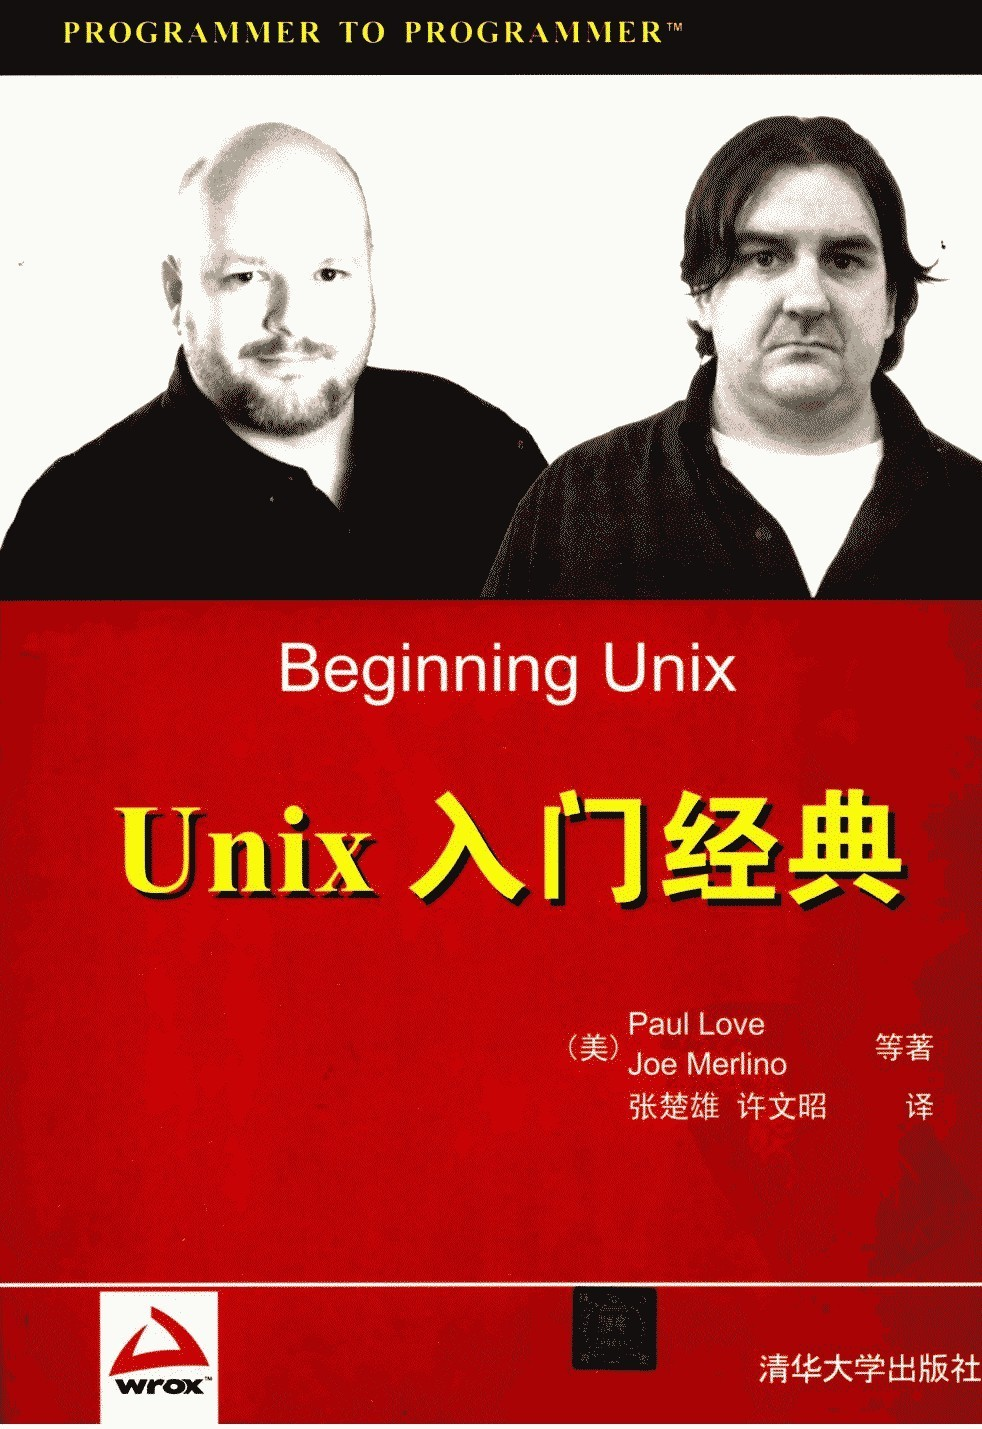
\includegraphics[width=0.4\textwidth]{c3.programming.linux.jpg}
  \end{figure}
\end{frame}

\section{学习方法}
\begin{frame}
  \frametitle{编程艺术 | 学习方法}
  \begin{block}{提问}
 学习编程的最佳方法是什么? 
  \end{block}
  \pause
  \begin{block}{回答}
    \begin{itemize}
      \item 取决于你要完成的任务
      \item 取决于你打算如何学习编程
      \item 取决于……
    \end{itemize}
  \end{block}
\end{frame}

\begin{frame}
  \frametitle{编程艺术 | 学习方法}
  \begin{block}{常见方法}
    \begin{itemize}
      \item 参加(XXX新手)培训班
      \item 阅读(XXX入门、\textcolor{gray}{30天学会XXX})书籍
      \item 死啃手册
      \item 拜师学艺
      \item 研究经典程序
      \item ……
      \item 组合多种方法
    \end{itemize}
  \end{block}
  \pause
  \begin{block}{\alert{五字真言}}
    \begin{itemize}
      \item 实践出真知!
      \item Experience is the best teacher.
      \item 不要只读书/看手册/读源代码,一定要亲自动手去编写、调试程序。
    \end{itemize}
  \end{block}
\end{frame}

\section{编写程序}
\begin{frame}
  \frametitle{编程艺术 | 编写程序 | \alert{基本流程(编辑-运行-修正)}}
  \begin{figure}
    \centering
    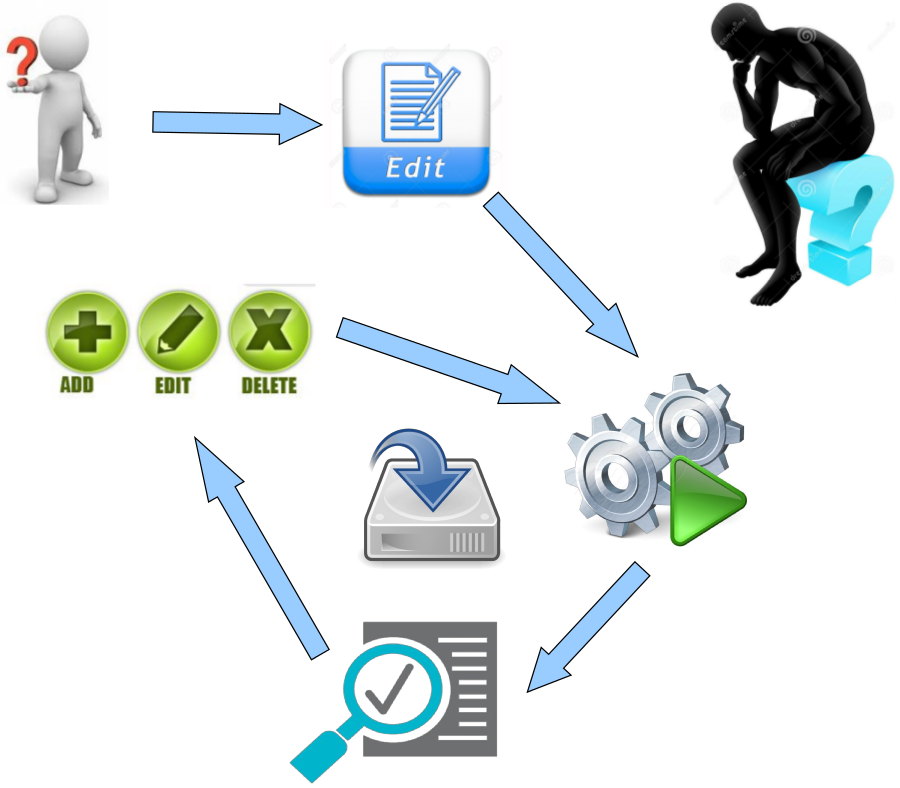
\includegraphics[width=0.72\textwidth]{c3.programming.cycle.png}
  \end{figure}
\end{frame}

\begin{frame}
  \frametitle{编程艺术 | 编写程序 | 版本控制}
  \begin{figure}
    \centering
    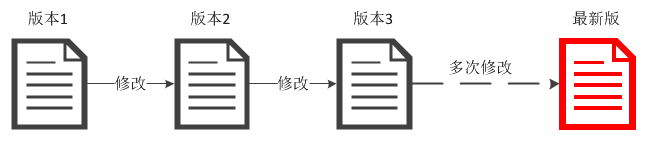
\includegraphics[width=0.7\textwidth]{c3.programming.version.01.png}\\
    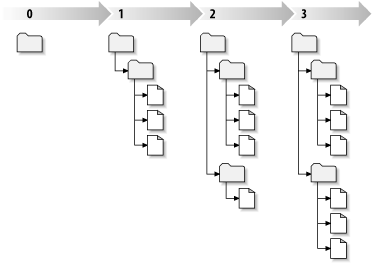
\includegraphics[width=0.8\textwidth]{c3.programming.version.02.png}\\
  \end{figure}
\end{frame}

\begin{frame}
  \frametitle{编程艺术 | 编写程序 | 版本控制}
  什么是版本控制?我真的需要吗?版本控制是一种记录若干文件内容变化,以便将来查阅特定版本修订情况的系统。\\
  \vspace{1em}
  如果你是位图形或网页设计师,可能会需要保存某一幅图片或页面布局文件的所有修订版本(这或许是你非常渴望拥有的功能)。采用版本控制系统(VCS,Version Control System)是个明智的选择。有了它你就可以将某个文件回溯到之前的状态,甚至将整个项目都回退到过去某个时间点的状态。你可以比较文件的变化细节,查出最后是谁修改了哪个地方,从而导致出现怪异问题,又是谁在何时报告了某个功能缺陷等等。使用版本控制系统通常还意味着,就算你乱来一气把整个项目中的文件改的改删的删,你也照样可以轻松恢复到原先的样子。但额外增加的工作量却微乎其微。\\
  \vspace{1em}
  许多人习惯用复制整个项目目录的方式来保存不同的版本,或许还会改名加上备份时间以示区别。这么做唯一的好处就是简单。不过坏处也不少:有时候会混淆所在的工作目录,一旦弄错文件丢了数据就没法撤销恢复。
\end{frame}

\begin{frame}
  \frametitle{编程艺术 | 编写程序 | 版本控制 | \textcolor{red}{Git}}
  Git是一个\textcolor{red}{分散式版本控制软件},最初由\textcolor{red}{林纳斯·托瓦兹(Linus Torvalds)}创作,于2005年以GPL释出。最初目的是为更好地管理Linux内核开发而设计。\\
  \vspace{1em}
  Git是用于Linux内核开发的版本控制工具。与CVS、Subversion一类的集中式版本控制工具不同,它采用了\textcolor{red}{分布式版本库}的做法,不需要服务器端软件,就可以运作版本控制,使得源代码的发布和交流极其方便。Git的速度很快,这对于诸如Linux内核这样的大项目来说自然很重要。Git最为出色的是它的合并追踪(merge tracing)能力。\\
  \vspace{1em}
  在Git中的绝大多数操作都只需要访问本地文件和资源,不用连网。因为Git在本地磁盘上就保存着所有当前项目的历史更新,所以处理起来速度飞快。
\end{frame}

\begin{frame}
  \frametitle{编程艺术 | 编写程序 | 版本控制 | Git | 原理}
Git和其他版本控制系统的主要差别在于,Git只关心文件数据的整体是否发生变化,而大多数其他系统则只关心文件内容的具体差异。\\
  \vspace{1em}
  这类系统(CVS,Subversion,Perforce,Bazaar等等)每次记录有哪些文件作了更新,以及都更新了哪些行的什么内容。\\
  \vspace{1em}
  Git并不保存这些前后变化的差异数据。实际上,Git更像是把变化的文件作快照后,记录在一个微型的文件系统中。每次提交更新时,它会纵览一遍所有文件的指纹信息并对文件作一快照,然后保存一个指向这次快照的索引。为提高性能,若文件没有变化,Git不会再次保存,而只对上次保存的快照作一链接。
\end{frame}

\begin{frame}[fragile]
  \frametitle{编程艺术 | 编写程序 | 版本控制 | Git | \textcolor{red}{范例}}
\begin{lstlisting}[language=sh]
# 安装Git
sudo apt install git-core
#sudo apt-get install git-core

# 使用帮助
man git
git --help
git help CMD

# 创建项目目录
mkdir ~/project
cd ~/project
\end{lstlisting}
\end{frame}

\begin{frame}[fragile]
  \frametitle{编程艺术 | 编写程序 | 版本控制 | Git | \alert{范例}}
\begin{lstlisting}[language=sh]
# 创建Git仓库(启动版本控制)
git init

# 创建编辑文件
vim script.pl
#print "Hello, world!";

# 添加需要进行版本控制的文件
git add script.pl
#git add .

# 提交改动信息
git commit -m "Say hello to the world."
\end{lstlisting}
\end{frame}

\begin{frame}[fragile]
  \frametitle{编程艺术 | 编写程序 | 版本控制 | Git | 范例}
\begin{lstlisting}[language=sh]
# 修改文件
vim script.pl
#把Hello替换成Bye

# 添加改动信息
git add .

# 提交改动信息
git commit -m "Bye to the world."

# 查看提交历史
git log

# 版本回退
git reset --hard ID #不需要全部ID,只需要有区分度的前几位即可
\end{lstlisting}
\end{frame}

\begin{frame}[fragile]
  \frametitle{编程艺术 | 编写程序 | 版本控制 | Git | \alert{范例}}
\begin{lstlisting}[language=sh]
# 创建test分支并切换过去
git checkout -b test
#相当于两步:git branch test; git checkout test

# 修改文件
vim script.pl
#添加一行:print "Bye, world!";

# 添加改动信息
git add .

# 提交改动信息
git commit -m "And bye to the world."
\end{lstlisting}
\end{frame}

\begin{frame}[fragile]
  \frametitle{编程艺术 | 编写程序 | 版本控制 | Git | \alert{范例}}
\begin{lstlisting}[language=sh]
# 切换回主分支
git checkout master

# 把test分支合并到主分支
git merge test
#可能需要手动修改后执行git add和git commit命令

# 删除test分支
git branch -d test
\end{lstlisting}
\end{frame}

\begin{frame}[fragile]
  \frametitle{编程艺术 | 编写程序 | 版本控制 | Git | \alert{范例}}
\begin{lstlisting}[language=sh]
# 查看状态
git status

# 查看提交日志
git log

# 查看修改内容
git diff

# 删除文件
git rm

# 查看/创建标签
git tag
\end{lstlisting}
\end{frame}

\begin{frame}[fragile]
  \frametitle{编程艺术 | 编写程序 | 版本控制 | Git | 范例}
\begin{lstlisting}[language=sh]
# 配置Git

#查看配置信息
git config --list

#彩色的 git 输出:
git config color.ui true
#显示历史记录时,只显示一行注释信息
git config format.pretty oneline

#配置个人信息等
git config --global user.name "Yixf"
git config --global user.email "yixf@example.com"
git config --global core.editor vim
\end{lstlisting}
\end{frame}

\begin{frame}[fragile]
  \frametitle{编程艺术 | 编写程序 | 版本控制 | Git | 范例}
\begin{lstlisting}[language=sh]
# 内置的图形化Git
gitk

# 忽略文件/文件夹
#将相关信息添加到.gitignore文件中
videos/
*.pdf
*.doc
\end{lstlisting}
\end{frame}

\begin{frame}
  \frametitle{编程艺术 | 编写程序 | 版本控制 | Git | \alert{范例}}
  \begin{figure}
    \centering
    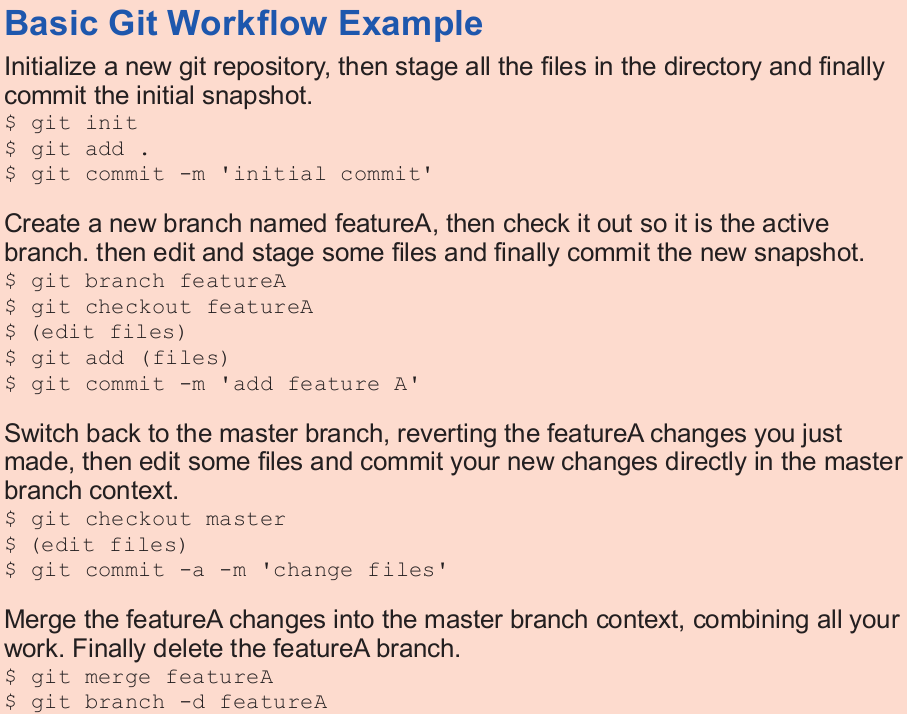
\includegraphics[width=0.8\textwidth]{c3.programming.git.png}
  \end{figure}
\end{frame}

\begin{frame}
  \frametitle{编程艺术 | 编写程序 | 版本控制 | \textcolor{red}{GitHub}}
  GitHub是一个共享虚拟主机服务,用于\textcolor{red}{存放使用Git版本控制的软件代码和内容项目}。\\
  \vspace{1em}
GitHub同时提供付费账户和免费账户。这两种账户都可以建立公开的代码仓库,但是付费账户也可以建立私有的代码仓库。除了允许个人和组织建立和存取代码库以外,它也提供了一些方便社会化软件开发的功能,包括允许用户跟踪其他用户、组织、软件库的动态,对软件代码的改动和Bug提出评论等。GitHub也提供了图表功能,用于显示开发者们怎样在代码库上工作以及软件的开发活跃程度。\\
\end{frame}

\begin{frame}
  \frametitle{编程艺术 | 编写程序 | 版本控制 | \textcolor{red}{GitHub}}
  \begin{columns}
    \column{0.5\textwidth}
截止到2016年4月,GitHub已经有超过一千四百万注册用户和三千五百万代码仓库。事实上已经成为了\textcolor{red}{世界上最大的代码存放网站}。\\
  \vspace{1em}
  GitHub里面的项目可以通过标准的Git命令进行访问和操作。同时,所有的Git命令都可以用到 GitHub项目上面。
    \column{0.4\textwidth}
    \begin{figure}
      \centering
      
\includegraphics[width=\textwidth]{c3.programming.github.logo.png}
    \end{figure}
\end{columns}
\end{frame}

\begin{frame}[fragile]
  \frametitle{编程艺术 | 编写程序 | 版本控制 | \alert{GitHub}}
\begin{lstlisting}[language=sh]
# 克隆仓库
#克隆本地仓库
git clone /path/to/repository
#克隆远程服务器上的仓库到本地
git clone username@host:/path/to/repository

# 把本地已有的仓库和服务器上的仓库关联起来
git remote add origin <server>

# 把本地库的内容推送到远程库
git push origin master

# 把远程库的内容更新到本地库
git pull
\end{lstlisting}
\end{frame}

\begin{frame}[fragile]
  \frametitle{编程艺术 | 编写程序 | 版本控制 | GitHub}
\begin{lstlisting}[language=sh]
# 克隆GitHub仓库到本地计算机(的当前目录下)
git clone https://github.com/Yixf-Education/project_Perl.git

# 进入项目目录
cd project_Perl
# 更新本地仓库(从GitHub中拉取最新变化)
#git pull

# 常规Git操作(...)
#vim script.pl; git add script.pl
#git commit -m "Fix typos in script.pl" 

# 推送修改(把本地修改上传到GitHub仓库中)
git push
\end{lstlisting}
\end{frame}

\begin{frame}
  \frametitle{编程艺术 | 编写程序 | 版本控制 | GitHub}
  \begin{figure}
    \centering
    \includegraphics[width=0.9\textwidth]{c3.programming.github.png}
  \end{figure}
\end{frame}

\begin{frame}
  \frametitle{编程艺术 | 编写程序 | 错误信息}
  \begin{itemize}
    \item 出错并不可怕!(【编程初期】出错是非常正常的。)
    \item 一定不要对错误信息视而不见!
    \item 从第一个错误开始,逐个进行修复。
    \item 必要时进行一定的猜测。
  \end{itemize}
\end{frame}

\begin{frame}[fragile]
  \frametitle{编程艺术 | 编写程序 | \alert{调试程序}}
  \begin{itemize}
    \item 使用Perl调试器:\verb|perl -d script.pl|。
    \item 在程序中加入print语句,输出中间值。
    \item 选择性地注释掉部分代码。
    \item 使用相关的模块:Benchmark,Data::Dumper,Smart::Comments,……
    \item 组合使用多种调试方法
    \item ……
  \end{itemize}
\end{frame}

\section{编程策略}
\begin{frame}
  \frametitle{编程艺术 | \alert{编程策略}}
  \begin{enumerate}
    \item 寻找现成的(免费/收费)程序:避免“重复发明轮子”
    \item 自己编写程序
      \begin{enumerate}
	\item 修改现成的程序(平时注意收集、整理程序)
	\item 充分利用已有模块,快速“拼凑”程序
	\item 从头编写完整的程序
      \end{enumerate}
    \item 请其他专家(无偿/有偿)编写程序
    \item 组合使用上述多种策略
  \end{enumerate}
  \pause
  \begin{block}{注意}
    有时修改现成的程序可能会比从头编写一个完整的程序还要困难!
    \begin{itemize}
      \item 背景知识
      \item 处理思路
      \item 编程风格
      \item ...
    \end{itemize}
  \end{block}
\end{frame}

\section{编程过程}
\begin{frame}
  \frametitle{编程艺术| 编程过程 | 实例}
  \begin{center}
    {\Large 计算一个DNA序列中调控元件的数目。}
  \end{center}
  \begin{figure}
    \centering
    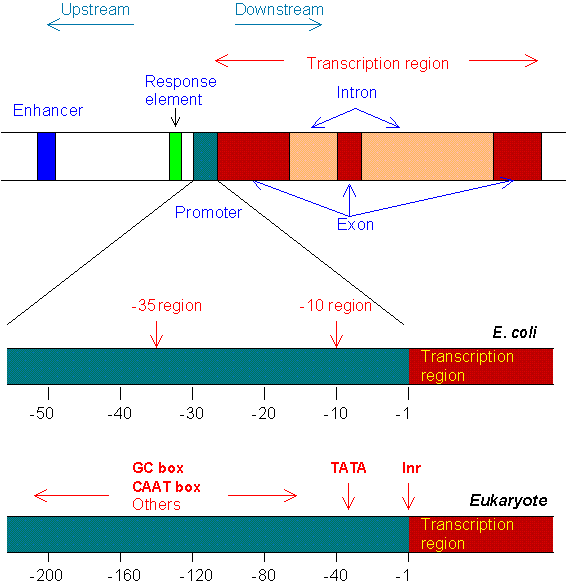
\includegraphics[width=0.55\textwidth]{c3.programming.re.01.png}
  \end{figure}
\end{frame}

\begin{frame}
  \frametitle{编程艺术 | 编程过程 | \alert{基本步骤}}
  \begin{itemize}
    \item 分析任务属性,对其进行充分的理解(数量、频率、时间等)
    \item 确定输入数据,对其进行充分理解(数据量、格式等)
    \item 对程序进行整理构思(算法、数据结构等)
    \item 确定输出数据,包括输出方法(文件、图形化展示、管道)、格式等
    \item 进一步改善整体构思,根据输入、输出等信息添加细节内容
    \item \textcolor{gray}{必要时}编写伪代码整理思路
    \item \textcolor{red}{最后}才是动手编写程序代码
  \end{itemize}
\end{frame}

\begin{frame}
  \frametitle{编程艺术 | 编程过程 | \alert{构思}}
  \begin{itemize}
    \item 程序构思:在实际编程前首先要完成的关键步骤
    \item 分析任务属性:任务数量、任务频率、解决任务的时间限制等
    \item 确定输入数据:数据来源(文件、输入等)、数据数量、数据校验(文件存不存在、格式对不对)等
    \item 选择正确/合适的算法(速度、优劣):针对每一个调控元件,在DNA序列中从头到尾进行查找;针对DNA序列的每一个位置,对每个调控元件进行查找
    \item 确定输出数据:输出形式、数据格式、人性化输出(用户提供文件名、易于解读……)等
    \item 选择编程范式:命令式编程(把一个大的问题/程序分割成多个微小、但却相互关联配合的部分/子程序),程序式编程,面向对象编程
    \item 编写伪代码:整理思路、优化构思、调整细节……
  \end{itemize}
\end{frame}

\begin{frame}
  \frametitle{编程艺术 | 编程过程 | \alert{总结}}
  \begin{itemize}
    \item 分析任务属性:任务数量、处理频率、时间限制等
    \item 确定输入输出:数据格式、数据量、数据校验、输出形式等
    \item 选择合适算法:算法速度、算法难易、对应数据结构等
    \item 编写伪代码:整理思路、优化构思、选择编程范式、调整细节等
    \item 编写程序代码:编辑、调试、运行、完善等
  \end{itemize}
\end{frame}

\begin{frame}
  \frametitle{编程艺术 | 编程过程 | 算法}
  在数学和计算机科学/算学之中,算法(algorithm)为一个计算的具体步骤,常用于计算、数据处理和自动推理。精确而言,算法是一个表示为有限长列表的有效方法。算法应包含清晰定义的指令用于计算函数。\\
  \vspace{1em}
  算法中的指令描述的是一个计算,当其运行时能从一个初始状态和初始输入(可能为空)开始,经过一系列有限而清晰定义的状态最终产生输出并停止于一个终态。\\
  \vspace{1em}
  程序所做的事情:获取文件、打开文件、读入数据、进行计算、输出结果;而算法就是此过程中计算的思路。
\end{frame}

\begin{frame}
  \frametitle{编程艺术 | 编程过程 | 伪代码}
  伪代码(pseudocode),又称为虚拟代码,是高层次描述算法的一种方法。它不是一种现实存在的编程语言;它可能综合使用多种编程语言的语法、保留字,甚至会用到自然语言。\\
  \vspace{1em}
  它以编程语言的书写形式指明算法的职能。相比于程序语言,它更类似自然语言。它是半形式化、不标准的语言。我们可以将整个算法运行过程的结构用接近自然语言的形式(这里可以使用任何一种作者熟悉的文字,例如中文、英文,重点是将程序的意思表达出来)描述出来。使用伪代码,可以帮助我们更好得表述算法,不用拘泥于具体的实现。\\
  \vspace{1em}
  人们在用不同的编程语言实现同一个算法时意识到,他们做出来的实现(而非功能)很不同。程序员要理解一个用他并不熟悉的编程语言编写的程序,可能是很困难的,因为程序语言的形式限制了程序员对程序关键部分的理解。伪代码就这样应运而生了。\\
  \vspace{1em}
  当考虑算法功能(而不是其语言实现)时,伪代码常常得到应用。计算机科学在教学中通常使用伪代码,以使得所有的程序员都能理解。
\end{frame}

\begin{frame}[fragile]
  \frametitle{编程艺术 | 编程过程 | 伪代码}
伪代码是介于自然语言和编程语言之间的一种“中间语言”。
  \begin{block}{代码}
\begin{lstlisting}[language=Perl]
sub getanswer {
  print "Type in your answer here :";  
  my $answer = <STDIN>;
  chomp $answer;
  return $answer;
}
\end{lstlisting}
\end{block}
\pause
\begin{block}{伪代码}
\begin{lstlisting}[language=]
getanswer
\end{lstlisting}
\end{block}
\end{frame}

\begin{frame}[fragile]
  \frametitle{编程艺术 | 编程过程 | \alert{伪代码}}
\begin{lstlisting}[language=Perl]
get the name of DNAfile from the user

read in the DNA from the DNAfile

for each regulatory element
  if element is in DNA, then
    add one to the count

print count
\end{lstlisting}
\end{frame}

\begin{frame}[fragile]
  \frametitle{编程艺术 | 编程过程 | \alert{注释}}
  \begin{itemize}
    \item 注释是源代码的一部分,旨在帮助用户/程序员理解程序
    \item 从 \verb|#|开始到行末的所有内容都被看做是注释,会被Perl解释器忽略掉
    \item 首行的 \verb|#!/usr/bin/perl|不是注释,不会被Perl解释器忽略掉
    \item 注释内容:程序的目的、整体构思、使用实例、细节注释等
    \item 牢记:代码不止是被计算机看的,也会被人查看
    \item 可以通过注释掉伪代码把它们保留在程序中
  \end{itemize}
\end{frame}

\section{编程真言}
\begin{frame}
  \frametitle{编程艺术 | 编程真言}
  \begin{block}{方法论——学习}
    \begin{itemize}
      \item 首次尝试某种事情时,最好从最基本的地方开始。你对\textcolor{red}{基础}理解得越好,以后你理解复杂问题时越轻松。
    \item \textcolor{red}{学习编程}和学习编程语言是截然不同的。应该掌握的不是答案,而是\textcolor{red}{思考方法}。学会靠自己的能力解决,而不是去记答案。
      \item 我们在做任何事情时,都需要100个小时后才能入门。
      \item 学习编程的两种方法:其一,是掌握工具,然后寻找能够用到的地方。其二,是找出要用的地方,然后掌握必要的工具。
      \item 任何事情都需要反复的\textcolor{red}{练习},编程也是同样的道理。
      \item 在程序的世界中,\textcolor{red}{英语}才是标准语言。
      \item 程序中的用语和习惯很多都受到了\textcolor{red}{数学}的影响。
      \item 编程中的思考方式和技术,不同语言之间的差别并不大。
      %\item 人们一般是在真正有需要时才会认真学习。在没有感到必要性时,我们是不会认真学习的。
      %\item 你要学的不是方法,而是思考方式。
      %\item 仅仅观察完成品,有时无法弄明白该如何制作,因为最重要的在于了解过程。
      %\item 最重要的不是知道“有这样的功能”,也不是学习这个功能的使用方法,而是理解这个功能在实现目标时起到的作用。
      %\item 在确定了想要做的东西后,需要学习的语言类型也就基本确定了。
    \end{itemize}
  \end{block}
\end{frame}

\begin{frame}
  \frametitle{编程艺术 | 编程真言}
  \begin{block}{方法论——理念}
    \begin{itemize}
      \item 在写任何程序之前最好先做个\textcolor{red}{计划}。想要达成目的,首先要思考从何处着手。
      \item 在拿到一个任务后,不要立即进行代码编写,而要先对任务进行\textcolor{red}{审视和分析},确定合适的策略后方可高效地解决问题。
      \item 无论是多么大的目标,都有其第一步。如果不实际着手,就无法开始。而且,关于第一步应该做什么,需要自己来思考。
      \item “先树立目标,再考虑手段”是编程时的基本思想。“先打造框架,再填充内容”的想法是非常基础的。
      \item 不建议在弄清问题前急于寻找工具。
      \item 在大多数情况下,比起编写时花费的时间,\textcolor{red}{修改错误以及进行维护时需要花费的时间更长}。
    \item 在尝试新内容的时候,尽量从\textcolor{red}{小的试验}开始。
      \item 现实生活中司空见惯的事情在程序的世界中并不一定理所当然。
      %\item 当出现“需要变成这种状态”的要求时,应该考虑“变成这样需要什么”。
      %\item 要回答“要做什么什么该怎么办”这个问题,必须先搞清楚这个“什么什么”才行。
      %\item 对比现状与目标的差距,继而找出前进方向的思考方式。
      %\item 认识到“程序有这样的结果,是因为我们写下的就是这样的内容”,然后推测问题所在。
      %\item 思考“想要得到预期的结果,必须要满足这样那样的条件,现在是否都满足了”,由此可以寻找出是否完成了必要的步骤。
      %\item 想要写出符合预期的内容,需要思考3点:
        %\begin{enumerate}
          %\item 试着运行一下,找到理想和现实的差异
          %\item 思考为什么会得到这样的现实
          %\item 思考怎样才能让理想与现实达成一致
        %\end{enumerate}
      %\item 人在第一次尝试的时候一般都会失败,无论精心多么周全的准备与难以避免失败的结局。所以提前做好失败的准备,然后尽早失败也并非坏事。
      %\item 当思考“这样就好了”时,最好思考“怎样才能变成这样”。
      %\item 在编程中,准备工作是十分重要的。有时稍微欠缺一些准备,就会为之后的工作增添许多烦恼。
    \end{itemize}
  \end{block}
\end{frame}

\begin{frame}
  \frametitle{编程艺术 | 编程真言}
  \begin{block}{方法论——思路}
    \begin{itemize}
      \item 当你受到挫折或者面临太大的挑战时:
        \begin{enumerate}
          \item \textcolor{red}{拆分}:把大问题拆成小问题,只考虑困难问题的一小部分
          \item \textcolor{red}{搁置}:把它放到一边一段时间,先不去理它,过几天再回来
        \end{enumerate}
    \item \textcolor{red}{一次只对程序做小的一点改动},这是因为我们最好一边做一边试验它是否好用。假如我们一次性把所有代码都写好,然后才发现它不工作,那我们要到哪里去找原因呢?
    \item 在我们希望推测程序的内部构造的时候,\textcolor{red}{稍加改造}后观察其变化是最基本的方法。
    \item 最好将\textcolor{red}{可变要素}控制为一个。如果同时修改两三个的话,就不知道是哪一项影响了最终的结果。
    \item 想要修正错误,从现在的运行\textcolor{red}{结果去推测原因}会比较快。
      \item 当我们要达成的事情比较复杂时,需要将达成的过程加以拆分,为每个过程设定目标,然后思考每个目标的达成手段。
      %\item 目标小一点的话,便于我们思考达成的手段。
      %\item 不断地进行分解和变形,从而找出可以立即开始着手的目标即可。最关键的就是找出“现在可以着手去做的事”。
      %\item 但是请记得确认,通过分解得到的目标是否符合原来的目的。
      %\item 编写程序的方法:通常,程序员会先创建类,而其中的函数什么也不做。先通过这种方式找出这个类应该做的事情,而不是马上进入到每个函数的细节中去。
      %\item 解决问题的一般思路:
        %\begin{enumerate}
          %\item 分析任务的原始数据和目标数据都涉及哪些数据,从而排除干扰数据,迅速定位有效数据。
          %\item 确定所要提取的有效数据后,观察有效数据的格式。通常利用分隔符可以较为便捷地构造出合适的模式以进行有效数据的提取。
          %\item 分析目标数据的层次关系及同层次数据颗粒间具有哪些关系,构造适合任务需求的数据结构。
          %\item 基于数据结构实现算法,完成任务。
        %\end{enumerate}
      %\item 在不知道某个构造的时候,最后对其稍加改造,观察一下效果。
      %\item 在进行新的尝试时,最好写出只包含所尝试的内容的代码。不要加入多余的要素,而致使程序过长。 
      %\item 在尝试新内容时,应将实验规模尽量控制得小一些。
      %\item 我们在尝试新功能的时候,都是尽量将程序缩减至最小。因为程序太大的话,再进行新尝试时会非常碍事。
      %\item 当我们遇到预想外的状况时,先从结果开始进行思考。
      %\item 当程序无法正常运行时,应该从结果出发推测原因。
      %\item 一点一点追加更便于编写。
      %\item 按照顺序进行思考 vs. 从结果出发进行思考
      %\item 不断将问题变形、分解为易于回答的问题,终会找出问题的解决方法。
      %\item 将“要达成目的该怎么办”转换为“什么情况下才算是达成目的”后,问题一般都会变得更具体。
      %\item 想要实现某个目的时,需要思考达成的方法。
    \end{itemize}
  \end{block}
\end{frame}

\begin{frame}
  \frametitle{编程艺术 | 编程真言}
  \begin{block}{方法论——补遗——通用}
    \begin{itemize}
      \item 精通的人往往无法理解不懂的人。
      \item 所谓的\textcolor{red}{最佳方法},会根据程序的不同、人的不同,甚至情绪的不同而发生变化。
      \item 进行准备工作也要分具体情况,避免做出多余的准备。到底应该做多少准备,需要根据具体情况而定。这需要经验的积累。
      \item 如果有精力的话,最好能想出两个以上的做法,将它们加以比较,然后选出其中较好的那个。如此一来就不需要陷入思维怪圈,而且做法行不通时也不用过于紧张。
      \item 永远正确的做法是不存在的。
      \item 当面对两个不同的方法时,一方独领风骚的情况非常少见。一般都是各有优势,需要根据当时的情况加以选择,即需要采取“扬长避短”的做法。
      \item 每个人都有着不同的生活状态,对事物抱着不同的看法、不同的感受。
      %\item 我们有时很容易忘记自己原本的目标。
      %\item 想要体会到一件事物的必要性,需要了解没有它时的窘境才行。较之用语言来形容,让你实际体验一下更有助于理解。
      %\item “将i或j作为循环次数。i在外侧,j在内侧”已经算是一种代码风格了。
      %\item 能够首先想到哪个方法,是根据运气和自己的经验决定的。
      %\item 如果你没养成“没有找到多个解决方案就不写程序”的习惯,可能就会选择首先想到的哪个“最差方案”了吧。
      %\item 程序不会突然就不按预期运行了。
      %\item 编程会受情绪的影响。状态好的时候可以轻松地写出复杂的程序。但回头看的时候大多内容会变得完全不明白,又改成更好懂的写法。人毕竟不是机器。
      %\item 程序不一定是越短越好。缩短程序只是编程中的手段罢了。
      %\item 乍一看完全没有天分的人不一定就没有天分,当事人说不擅长也并不代表真的不擅长。
      %\item 重用会使你的代码变得简短而易读。
      %\item 如果我们在一个地方写了太多的代码(比方说在一个函数里),我们会让代码变得难于理解。
      %\item 在文本处理中,第一步操作几乎都是进行有效数据的提取。如果有效数据是具有一定格式的,花点时间进行格式观察是非常必要的。
      %\item 有意义的答案能告诉你“先做这件事”。
      %\item 无论多么易懂,一旦量太大就不简单了,反而非常困难。
      %\item 由于缩减程序很费功夫,因此有时候为了了解运行状况,需要尽快让程序运行起来,那时可能就需要对代码进行复制。然而,这种不负责任的代码,还是需要尽快修改好才是。
      %\item 在程序中添加新要素前,最好想想能不能将程序写得更简短明了一些。
      %\item 当遇到没有新工具就无法解决的困难时,要考虑一下引入怎样的工具才能解决这个问题。如果正好有这样的工具,那么顺手取来使用即可。如果没有,要么制作出来,要么选择其他方法,要么干脆放弃。
      %\item 编程语言的规则是为了便于使用而设定的,有时可能会稍微有些改变,和现实世界中的规则是一个道理。
      %\item 如何取得“所花费的功夫”和“程序易读性”之间的平衡是你的自由,但就我个人的经验而言,我宁愿多花费一些时间让代码更易懂。
      %\item 不是任何时候都越小越好,能够快速清晰地看出有没有写对才是重中之重。
      %\item 特殊情况越多就越容易出错,就好似“特例多的规则不好懂”一样。
      %\item 与其将规则复杂化,还不如使用较为麻烦的方案。
      %\item 一般而言,如果只能找打一种方法,就意味着还不到写代码的时候。
      %\item 技术含量高的不一定永远都是最好的。简单的写法可能在运行效率上差一些,但是易写易读,不容易出错,出错时也容易修正。
      %\item 一般而言,“麻烦”是有错误的征兆。在程序的世界中,“麻烦”是非常重要的信息,决不能忽略。
      %\item 最好在想到两种以上的方法后再开始编程。
      %\item 从结果开始考虑,结果一样的话做法奇怪也没关系。
      %\item 什么样的程序更易懂,取决于个人的技术水平。
      %\item 如果不实际进行编写就能推想出来的话,最好事先进行推想。这样既有助于缩短时间,也方便在编写时把握好整体的平衡性。
      %\item 当程序中存在大量的有条件运行时,我们通常会通过事先存入存储区的方法来消除有条件运行。
      %\item 与其每次都运行复杂的程序,不如事先将大量的计算结果存入表格中,每次使用时再找出所需信息。
      %\item 编程不过是一个手段罢了。
      %\item 没有找到多个解决方案时就不写程序。
      %\item 当编写较大的程序时,可以对代码加以重复利用。
      %\item 与其在多年积攒的笔记中寻找答案,直接当场解题可能来得更快。
      %\item 在编程中,知道如何“敷衍一下”也是一项编程技术。
      %\item “只要结果相同就不在乎结局方法”的情况非常普遍。
      %\item 没有名字的东西越多,程序越难理解。
      %\item 很多时候不亲自试一试的话是无法了解详情的。
      % \item 一般而言,从头开始做的话更好一些。没有过多的负担,思路更清晰。
      % \item 首先做出一部分,随后加以修改和组合的话,编写起来则更容易,但其结果很难是“最简洁的方法”。
      % \item 代码并不是越短越好。
      % \item 问题能不能得到解决,取决于提问的内容。
      % \item 不在技术上过多纠缠,反而可能帮助我们看清本质。
      % \item “为了什么而编程”这个问题非常重要。
    \end{itemize}
  \end{block}
\end{frame}

\begin{frame}
  \frametitle{编程艺术 | 编程真言}
  \begin{block}{方法论——补遗——编程}
    \begin{itemize}
      \item 程序不是按你想的运行,而是按你写的运行。
      \item “开始无法按照预期运行,然后一遍遍地修改再试”——这种循环是不可避免的。先写再修正,再写再修正……
      \item 适合编程的人和不适合编程的人之间存在显著的差异。差异不在于记忆力的强弱、脑子的灵活程度或者计算能力的高低这些单纯的内容,而在于思考方式与世界观的差别。与其说谁优谁劣,不如说是\textcolor{red}{性格或者个性}的问题。
      \item 编程需要养成的\textcolor{red}{习惯}:
        \begin{itemize}
          \item 从结果出发
          \item 提问的方法非常重要,需要好好对问题加以变形
          \item 带着目的,将其分解为更容易立即着手的小目标
          \item 对出现的手段是否符合自己的目的加以确认
          \item 准备多个选项,进行比对、选择
        \end{itemize}
      % \item 编写程序所需的时间,会随着技术水平的提高渐渐缩短。
    \end{itemize}
  \end{block}
\end{frame}

\begin{frame}
  \frametitle{编程艺术 | 编程真言}
  \begin{block}{计算机科学家}
    \begin{itemize}
      \item 计算机科学家与数学家类似,他们使用形式语言来描述理念(特别是计算);与工程师类似,他们设计产品,将元件组装成系统,对不同的方案进行评估选择;与自然科学家类似,他们观察复杂系统的行为,构建科学家说,并检验其预测。
      \item 作为计算机科学家,最重要的技能就是\textcolor{red}{问题求解}。问题求解是发现问题、创造性地思考解决方法以及清晰准确地表达解决方案的能力。实践证明,学习编程的过程,正是训练问题求解能力的绝佳机会。
    \end{itemize}
  \end{block}
\end{frame}

\begin{frame}
  \frametitle{编程艺术 | 编程真言}
  \begin{block}{程序员}
    \begin{itemize}
      \item 好的程序员不愿意重复做同一件事情,应尽全力找出省事的方案。
      \item 勤奋的程序员是不对的。最终能够成功的,是知道如何\textcolor{red}{偷懒}的人。
      \item \textcolor{red}{自我探索并解决问题的精神}被共认为是一个软件工程师应有的基本素质之一。 
      \item \textcolor{red}{新手}在进行编程时,或者编写复杂的内容时,就应该一步一个脚印,频繁地进行测试。而\textcolor{red}{专家}在编写简单的内容时,一次进行大量的改造反而有助于把握好整体结构,也便于提高效率。
      %\item 程序写的太长可是程序员的罪过。
      %\item 程序员在遇到麻烦的事情时,必须想出省事的方法。
    \end{itemize}
  \end{block}
\end{frame}

\begin{frame}
  \frametitle{编程艺术 | 编程真言}
  \begin{block}{计算机}
    \begin{itemize}
      \item 计算机是人的工具,只有人才知道他自己想让计算机做什么。
      \item 计算机就是对一切内容都通过计算进行处理的东西,计算之外的内容完全不明白。
      \item 计算机是由“运行程序的装置”和“大量的内存”这两者组成的。
      \item 计算机是按照程序中的内容操纵存储区,让外部设备运转的设备。
      \item 计算机只能理解数字。
      \item 计算机无非就是一种“\textcolor{red}{自动化设备}”,也就是处理复杂内容的帮手。当你感到麻烦时,不妨想想能否交给计算机来处理。“麻烦”在编程中是极为重要的信号。
    \end{itemize}
  \end{block}
\end{frame}

\begin{frame}
  \frametitle{编程艺术 | 编程真言}
  \begin{block}{程序}
    \begin{itemize}
      \item 计算机程序是一组让计算机执行某种动作的指令。计算机程序就是一系列告诉没有知觉的硬件做什么事情的命令。程序有点像\textcolor{red}{思想}。思想告诉你做什么,计算机程序告诉计算机做什么。
      \item 程序究竟能做什么?它只能修改保存在存储区中的数字。程序就是由操纵存储区的命令组合而成的。程序就是告诉计算机“按什么顺序让哪个存储区记住哪个数字”的东西,它所能做的只有\textcolor{red}{操纵存储区}罢了。
      \item 所谓程序,就是记录着如何改变存储区所存数值的文章。通过操纵存储区,能够对与存储区相连的设备施加影响。程序是按照“以什么顺序”“向哪个存储区”“保存哪个数字”写下的东西。
      \item 软件就是计算机程序的集合。
      % \item 程序是指一组定义如何进行计算的指令的集合。这种计算可能是数学计算,如解方程组或者查找多项式的根,也可以是符号运算,如搜索和替换文档中的文本,或者图形相关的操作,如处理图像或播放视频。
      %\item 软件就是一组计算机程序。
      %\item 程序就是一系列指令,告诉计算机做什么事情。
      %\item 程序是依照编程语言的规则写成的。程序是根据某种规则写就的“奇妙文章”程序就是各种类型的语句按照语言文法规则组合在一起的代码块。
      %\item 程序代码就是变量按照规定的语法组织在一起的。在代码运行时,变量按照设计好的流程变换变量内容。
      %\item 程序会一直运行,不会停留在同一行。运行完某一行后,就会接着移至下一行并运行,如此反复。
      %\item 程序不一定是从上向下进行阅读的东西。在包含局部程序的程序中,运行顺序不一定是自上至下。
    \end{itemize}
  \end{block}
\end{frame}

\begin{frame}
  \frametitle{编程艺术 | 编程真言}
  {\footnotesize
  \begin{block}{编程与编程语言}
    \begin{itemize}
      \item 编程会培养\textcolor{red}{创造能力、逻辑能力和解决问题的能力},从中学到的技巧对于学校和工作都很有用。学习编程是一种很好的\textcolor{red}{思维训练}。
      \item 一种编程语言就是一种特定的与计算机\textcolor{red}{交谈的方式},它使用计算机和人都能理解的指令。
      \item 程序设计过程就是\textcolor{red}{加工处理数据}的过程。输入数据给程序,经过程序处理后,输出处理结果。
      \item 在不同的编程语言中,程序的细节有所不同,但几乎所有编程语言中都会出现以下几类\textcolor{red}{基本指令}:
        \begin{description}
          \item[输入] 从键盘、文件或者其他设备中获取数据
          \item[输出] 将数据显示到屏幕,保存到文件中,发送到网络上等
          \item[数学] 进行基本数学操作,如加法或乘法
          \item[条件执行] 检查某种条件的状态,并执行相应的代码 
          \item[重复] 重复执行某种动作,往往在重复中有一些变化 
        \end{description}
      \item 可以把编程看作一个将大而复杂的任务分解为更小的子任务的过程,不断分解,直到任务简单到足以由基本指令组合完成。
      % \item 编程语言是人们为了表达计算过程而设计出来的形式语言。语法规则有两种,分别适用于记号和结构。记号是语言的基本元素,结构指定记号所组合的方式。
      % \item 同一种语言总不能适合所有的任务,所以不要惧怕在你的电脑上用不同的方式编程。
      % \item 在计算机编程中,每次你输入同一个命令它都应该完全以同样的方式工作。
      %\item 形式语言的密度远远大于自然语言,其结构和细节都非常重要。
      % \item Perl/Python中的关键字是有特殊意义的词。
    \end{itemize}
  \end{block}
}
\end{frame}

\begin{frame}
  \frametitle{编程艺术 | 编程真言}
  \begin{block}{编程的本质}
    \begin{itemize}
      \item 要编写程序,就必须知道编程语言的规则。语法指的是程序中文字的组织和顺序。虽然语法和词汇的使用方法不得不记,但仅仅记住这些是无法写出文章的。记住编程语言和记住\textcolor{red}{编程方法}不是一回事。
      \item 计算机上的诸多功能,都是通过\textcolor{red}{用程序修改存储区}的方法来实现的。
      \item 操纵外部装置需要使用存储区,使用外部装置进行操作时还是要用存储区。向外部装置传递信息或者发出指示的时候,只要操纵存储区即可。
      \item “如果这样,如果那样”这种逻辑,在计算机看来,不过是数字之间加减乘除的结合罢了。
      \item 编程的本质:不断在“易懂但量大”和“复杂却量少”之间挣扎。
      % \item 在不影响结果的同时改善代码运行效率和可读性的方法在编程中称为“(代码)重构”。
      % \item 值是程序操作的最基本的东西,如一个字母或者数字。
      %\item 数学中的变量,完全可以用存储区来实现。
      %\item 编写程序时,当然是越短却轻松,存储区用得越少越轻松。
      %\item 在使用编程语言进行编程之前,你首先需要准备必要的软件。
      %\item 让“一行运行得慢一些”是不可能的。
      %\item 对于计算机而言,不能直接移动到下一行时会增加工作量,所以会浪费很多的时间。
    \end{itemize}
  \end{block}
\end{frame}

\begin{frame}
  \frametitle{编程艺术 | 编程真言}
  \begin{block}{算法与数据结构}
    \begin{itemize}
      \item 编程的核心是数据结构。\textcolor{red}{程序 = 数据结构 + 算法}
      \item 所谓数据结构就是指一类数据的内部构成,即一类数据由那些成员数据构成,以什么方式构成,有什么特点。
      \item 算法好比武术中的种种套路,告诉你先干什么,后干什么。数据结构却好比我们手中的兵刃,性能好坏导致使用效果大相径庭。
      \item 在开始一个程序代码的编写前,选择合适的数据结构可以帮助我们更好地完成和实现目标功能,并且有助于后期算法的实现。
      %\item 一个复杂的数据结构可以比作一件复杂的武器。 
    \end{itemize}
  \end{block}
\end{frame}

\begin{frame}
  \frametitle{编程艺术 | 编程真言}
  \begin{block}{注释}
    \begin{itemize}
      \item 在复杂和难以理解的地方加入\textcolor{red}{注释}也是编程的一种好习惯。好的注释可以充当程序的说明文档。
      \item 标有注释的地方,就是没有注释便难以理解的地方。不得不添加注释,并不是件好事。注释毕竟不是程序,不但麻烦而且难以信赖。
      \item “虽然修改了程序,但是没有修改注释”的情况屡见不鲜。这会导致注释中的内容根本不正确,比没有注释更可怕。注释是在没有其他更好的手段进行说明时不得已而采取的措施。
      \item 程序过长比较难懂时,才必须写下类似于“这里的程序是这种作用”的注释。在这种情况下,我们可以通过使用局部程序,做到即使不使用注释也能让程序更易懂。
      \item 如果你必须要在某处写下注释,就可能暗示着那里存在问题。
      %\item 随意的规则与注释相同,毫无约束力。
    \end{itemize}
  \end{block}
\end{frame}

\begin{frame}
  \frametitle{编程艺术 | 编程真言}
  \begin{block}{调试}
    \begin{itemize}
      \item 在修复程序时,需要考虑“怎样的错误才会导致这样的结果”。
      \item 纠错方法:其一,是观察现有代码,找出错误。其二,是通过观察程序的运行结果,推理出程序的问题所在。
      \item 出现错误时,我们不能单单询问“该怎么办才能改好”,因为这样做事情不会有任何进展。此时可以导入“从结果出发记性思考”的方法,将问题变形为“要出现这样的结果,程序必须存在怎样的错误”后,才算是朝着问题的解决前进了一步。
      \item \textcolor{red}{学习调试}可能会带来挫折感,但它是一个有价值的技能,并在编程以外还有很多用途。
      \item 一个程序中可能出现3中类型的错误:语法错误、运行时错误和语义错误。
      \item 每当你试验新的语言特性时,应当试着故意犯错。这种试验会帮你记住所读的内容,也能帮你学会调试,因为这样能看到不同的出错消息代表着什么。现在故意犯错总比今后在编程中意外出错好。
      % \item 思考一下“无法达成目的的条件是什么”或许同样有用,这样可以搞清楚都有哪些障碍。
    \end{itemize}
  \end{block}
\end{frame}

\begin{frame}
  \frametitle{编程艺术 | 编程真言}
  \begin{block}{变量}
    \begin{itemize}
      \item 变量是计算机程序中用来保存东西的一种方式。
      \item 变量指一个存储信息的地方,就像贴在东西上的标签。
      \item 变量就是一种给事物加标签的方法,从而让我们以后可以使用它们。
      \item 变量就是一个可以存储常量的\textcolor{red}{存储器}。一个变量就像是计算机内存中的信息\textcolor{red}{标签}。
      \item 选择什么样的名字取决于你需要让这个变量名有多么大的含义。
      \item 作用域是指一个变量的可见范围。变量的作用域控制它在函数内外的可见性。
    \end{itemize}
  \end{block}
\end{frame}

\begin{frame}
  \frametitle{编程艺术 | 编程真言}
  \begin{block}{条件与循环}
    \begin{itemize}
      \item 条件就是用来做比较的程序语句。
      \item “有条件运行”说到底不过是“最多只能循环1次的循环”。
      \item 有条件运行本身不过是循环的一种,但实际进行编程时,循环和有条件运行则会被视为不同的东西。
      \item for循环是针对指定长度的循环,而while循环则用于你事先不知道何时停止循环的情况。
      \item 一般而言,缩短程序就意味着需要增加同一行的重复运行次数。能用循环的时候就用循环,减少行数,增加同一行的运行次数。
      \item 在使用循环时,如何平衡“简单却冗长”与“复杂却简短”这两者的关系,是个永恒的话题。这里没有正确答案,需要根据具体情况进行具体分析,找出最有利的方案。
      %\item 最简单的缩减方法,就是对代码中的相同内容进行删减。
      % \item 写很多if或者elif语句但是都返回相同的值,这并不是好的变成方法。可以用括号把条件括起来,用or关键字来连接它们,这样可以让代码变得短一些。
      % \item 当程序中存在大量的有条件运行时,通过使用表格,有助于编写出简明的代码。
    \end{itemize}
  \end{block}
\end{frame}

\begin{frame}
  \frametitle{编程艺术 | 编程真言}
  \begin{block}{函数}
    \begin{itemize}
      \item 函数就是让Perl/Python做某些事情的一段代码。它们是\textcolor{red}{重用代码}的一种方式。
      \item 创建函数来重用代码,使用类和对象把代码划分成小块。函数还可以按模块的方式组织起来。
      \item 函数就是一个给出了调用接口的自包含模块。函数名其实就是函数的标识。
      \item 某些功能用函数实现可以有以下好处:
        \begin{itemize}
          \item 可以使程序逻辑清晰,代码可读性好
          \item 用一个可读性好的名字给函数命名,可以帮助理解程序代码的含义
        \end{itemize}
    \end{itemize}
  \end{block}
\end{frame}

\begin{frame}
  \frametitle{编程艺术 | 编程真言}
  \begin{block}{模块}
    \begin{itemize}
      \item 在Perl/Python中,模块是给别的程序提供有用的代码的一种方式。
      \item Perl/Python的模块就是一些函数、类和变量的组合。模块用来把函数、变量,以及其他东西分组,组织成更大的、更强的程序。
      \item 模块要先被引用/载入然后才能使用。
      \item 使用扩展模块通常采用\textcolor{red}{示例驱动方法},即参照扩展模块使用说明文档中的示例,通过简单改造示例的方法即实现我们自己期望的功能。
    \end{itemize}
  \end{block}
\end{frame}

\begin{frame}
  \frametitle{编程艺术 | 编程真言}
  \begin{block}{引用与子程序}
    \begin{itemize}
      \item 引用就是一个指向某个数据结构(可以是一个简单变量、一个数组或一个哈希等)的标量值,通过引用可以间接访问原始数据。一个引用中所存储的是其引用对象的地址。
      \item 通过使用引用,不但可以缩减代码,还可以方便理解程序。
      \item 使用局部程序可以缩短程序。有时使用局部程序虽然不能缩短程序,但却能让程序更易懂。
      \item 当你做出新的局部程序时,建议你使用类似的小程序来检查代码是否正确。需要寻找错误时,当然是程序越小越方便。
      \item 局部程序是编写大型程序时的利器。
    \end{itemize}
  \end{block}
\end{frame}

\begin{frame}
  \frametitle{编程艺术 | 编程真言}
  \begin{block}{面向对象编程}
    \begin{itemize}
      \item \textcolor{red}{对象是程序组织代码的方法},它把复杂的想法拆分开来使其更容易被理解。\textcolor{red}{类是一组函数和变量}。对象是由“类”定义的,可以把“类”当成一种把对象分组归类的方法,可以把一个对象想象成是一个类家族中的一员。
      \item 类和对象是给函数分组的好方法,它们帮助我们把程序分成小段来分别思考。
      \item “特征”就是一个类家族中的所有成员(还有它的子类)共同的特点。
      \item 有些类中的函数什么也不做,这其实在编程中很常见。某种意义上讲,这是一种共识,确保一个类的所有子类都提供同样的功能,尽管有时子类中的函数什么也不做。
      \item 不必强迫自己去理解面向对象。思考方式到头来不过是一种工具罢了。面向对象是工具,面向对象的程序设计语言也是工具。最重要的是“面向对象能为我们做什么”,而不是“面向对象是什么”。
    \end{itemize}
  \end{block}
\end{frame}

\begin{frame}
  \frametitle{编程艺术 | 编程真言}
  \begin{block}{其他}
    \begin{itemize}
      \item 在计算机显示器上看到的所有东西都是由\textcolor{red}{像素}组成的,它们是很小的、方块的点。一个像素就是屏幕上的一个点,也就是可以表现出的最小元素。
      \item 所谓\textcolor{red}{比较字符的大小},其实就是比较它们在计算机内部存储编码的大小。字母是按照字母表顺序排列的,并且小写字母排列在大写字母的后面。
      \item 先画一张图,再画一个稍稍有点变化的图,这就让人感觉它在移动。这就是\textcolor{red}{动画}。
      \item 实际上,你计算机上的所有东西都是以文件的形式保存。
      \item 通过参数化运行方式,程序处理数据的方式变得更加灵活,做到了代码与具体文件名无关,代码运行的方式通过参数开关进行控制。
      \item 在计算个数时从1开始比较好,既自然又方便。除了计算个数以外,都是从0开始比较方便。
      % \item 字符串是由字符构成,模式是对字符串的概括性的描述,模式匹配就是从制定字符串中寻找符合制定模式的子串。通过模式匹配方式,我们也能进行数据格式的判定。
      % \item 代码中的语句块就是组合在一起的一组程序语句。
      % \item 程序员经常在程序的开头就定义变量。
      % \item “用户输入”就是人在键盘上输入的内容。
      % \item 坐标定义了一个平面上像素的位置。角度就是一种对圆周上的距离的度量。
      % \item 要记得一边写一边保存。
      %\item 像素是你计算机屏幕上的一个点,那是计算机能画出的最小的点。
      % \item 网络爬虫需要完成一下主要功能:
      %   \begin{enumerate}
      %     \item 文件或页面下载
      %     \item 页面内嵌URl抽取
      %     \item 页面清洗
      %     \item URl及数据管理
      %   \end{enumerate}
    \end{itemize}
  \end{block}
\end{frame}

\section{回顾与总结}
\subsection{总结}
\begin{frame}
  \frametitle{编程艺术 | 总结}
  \begin{block}{知识点}
    \begin{itemize}
      \item 学习编程的方法:培训班、读书、看手册、拜师、研究程序、……
      \item 编程的基本流程:编辑-运行-修正
      \item 版本控制:Git,GitHub
      \item 调试程序:调试器、print、注释、模块、……
      \item 编程策略:找现成的程序、自己编写程序、请别人帮忙、……
      \item 编程的基本步骤:构思(输入、算法、输出)、编程
      \item 编程前:伪代码;编程中:注释
    \end{itemize}
  \end{block}
  \pause
  \begin{block}{技能}
    \begin{itemize}
      %\item 能够自学一门编程语言
      \item 熟练应用编程的基本策略、步骤和流程
      \item 能够使用Git和GitHub进行版本控制
      \item 能够用不同的方法调试程序
      %\item 能够针对不同的问题采用不同的编程策略
      %\item 能够熟练撰写伪代码
    \end{itemize}
  \end{block}
\end{frame}

\subsection{思考题}
\begin{frame}
  \frametitle{编程艺术 | 思考题}
  \begin{enumerate}
    \item 总结学习编程语言的方法。
    \item 编写程序的基本流程是什么?
    \item 如何使用Git进行版本控制?
    \item 总结调试程序的方法。
    \item 总结常用的编程策略。
    \item 编程的基本步骤是什么?需要构思哪些内容?
    \item 使用伪代码和注释有哪些优势?
  \end{enumerate}
\end{frame}

\begin{frame}
  \frametitle{下节预告}
  \begin{block}{编程相关}
    回顾shell/Perl中的以下知识点:
    \begin{itemize}
      \item 变量
      \item 数组
    \end{itemize}
  \end{block}
  \begin{block}{生物学相关}
    回顾生物学中的以下知识点:
    \begin{itemize}
      \item DNA的组成
      \item DNA的转录
      \item DNA的反向互补
      \item 蛋白质的组成
    \end{itemize}
  \end{block}
\end{frame}



\section*{Acknowledgements}
\begin{frame}
  \frametitle{Powered by}
  \begin{center}
    
\includegraphics[width=9cm]{power.png}
  \end{center}
\end{frame}

\end{document}

